% fixture: tikz/plots-pdftex
% oracle: pdflatex
% tier: T3
% engine: document
% specials: compare
% covers: plot coordinates (moved and lined to, a node's anchor among them), plot (\x,{f(\x)}) over a domain and samples (sin with r, products, exp, a parametric circle, samples at, variable=), marks (*, +, x and plotmarks' o, mark size, mark options, only marks), the plot's last point as the current one; ellipse nodes of shapes.geometric (anchors, borders, minimum height, a label and an edge)
% issue: #326
\documentclass{article}
\usepackage{tikz}
\usetikzlibrary{plotmarks,shapes.geometric}
\begin{document}
\noindent Plots: 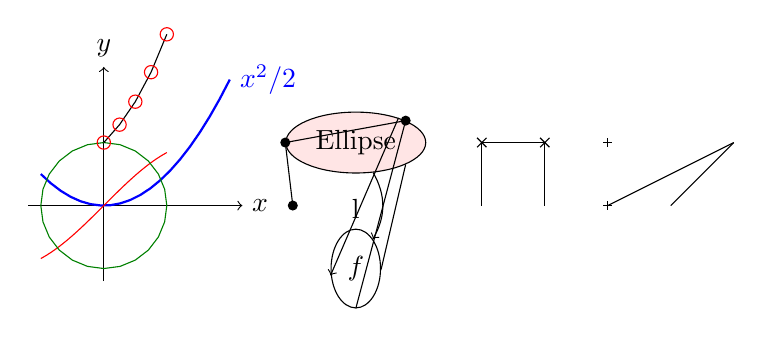
\begin{tikzpicture}[scale=0.8]
  \draw[->] (-1.2,0) -- (2.2,0) node[right] {$x$};
  \draw[->] (0,-1.2) -- (0,2.2) node[above] {$y$};
  \draw[blue,thick,domain=-1:2,samples=20] plot (\x,{\x*\x/2}) node[right] {$x^2/2$};
  \draw[red,domain=-1:1] plot (\x,{sin(\x r)});
  \draw[green!50!black] plot[domain=0:360,samples=25] ({cos(\x)},{sin(\x)}) -- cycle;
  \draw[variable=\t,domain=0:1,samples=5,mark=o,mark options={red,scale=1.5}] plot (\t,{exp(\t)});
  \node[ellipse,draw,fill=red!10] (e) at (4,1) {Ellipse};
  \node[ellipse,draw,minimum height=1cm,label=above:l] (f) at (4,-1) {$f$};
  \draw plot[mark=*] coordinates {(3,0) (e.west) (e.north east)} -- (f.south);
  \draw[mark=x,mark size=3pt] (6,0) -- plot coordinates {(6,1) (7,1)} -- (7,0);
  \draw plot[only marks,mark=+] coordinates {(8,0) (8,1)} plot[samples at={0,0.5,...,2}] (\x+8,\x/2);
  \draw[samples=1,domain=0:1] plot (\x+9,{\x}) plot[domain=1:1] (\x+9,2);
  \draw[->] (e) edge[bend left] (f) (e.south east) -- (f.mid east) (e.30) -- (f.base west);
\end{tikzpicture}
\end{document}
